\section{Modos de operação}
\label{sec_modos_operacao}

Durante a simulação da missão de \gls{rvdb}, o modelo dinâmico do sistema opera em dois modos distintos, definidos de acordo com a etapa da aproximação e a distância relativa em relação ao alvo.

No modo não-operacional, o \gls{mr} permanece travado e a dinâmica da espaçonave é representada apenas pelo modelo de corpo rígido. 
Nesse regime, a dinâmica e a atitude são descritas pelas equações de Euler, considerando somente a matriz de inércia da espaçonave e os torques aplicados pelo sistema de controle de atitude.

No modo operacional, o \gls{mr} passa a se movimentar e a dinâmica do sistema passa a considerar o acoplamento entre a espaçonave e o manipulador. 
Nesse caso, a modelagem dinâmica passa a utilizar a formulação baseada nas equações de Lagrange, permitindo representar os efeitos das movimentações articulares do manipulador sobre a atitude da espaçonave.

A Tabela~\ref{tab_modos_operacao} apresenta o resumo dos modos de operação considerados na simulação.

\begin{table}[H]
\centering
\caption{Modos de operação utilizados no modelo de simulação.}
\label{tab_modos_operacao}
\begin{tabular}{c p{9cm}}
\hline
Modo & Descrição \\
\hline
0 & Modo não operacional: O \gls{mr} permanece travado e a dinâmica da espaçonave é representada pelo modelo de corpo rígido baseado nas equações de Euler. \\
\hline
1 & Modo operacional: O \gls{mr} é destravado e a dinâmica do sistema passa a considerar o acoplamento entre a espaçonave e o manipulador, utilizando a formulação de Lagrange. \\
\hline
\end{tabular}
\end{table}

A lógica responsável pela determinação do modo de operação foi implementada no ambiente Simulink, conforme ilustrado na Figura~\ref{fig_modo_operacao}. 
Nesse bloco, o valor do modo é utilizado para selecionar qual modelo dinâmico será empregado durante a simulação.
Foi utilizado $0$ para o modo não-operacional e $1$ para o modo operacional.

\begin{figure}[H]
\centering
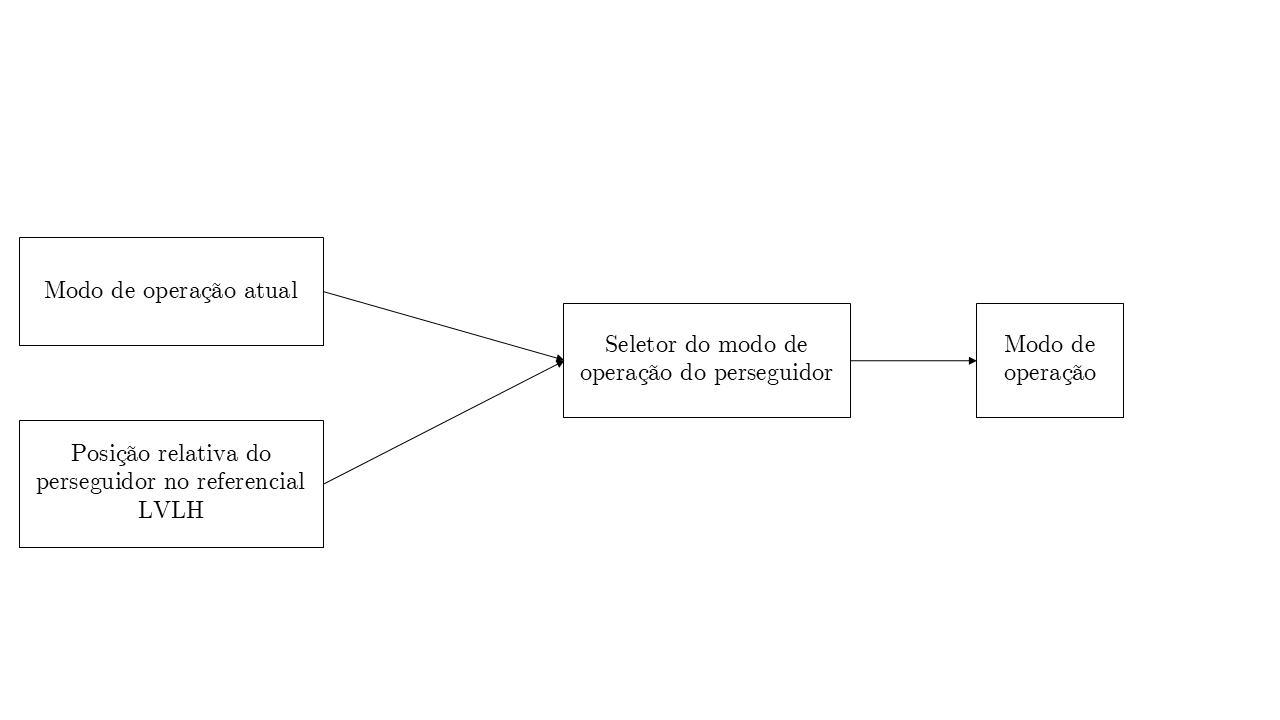
\includegraphics[width=1\linewidth]{3 Procedimento simulacao/Imagens simulink/app_final_modo_operacao.png}
\caption{Definição do modo de operação do modelo dinâmico.}
\label{fig_modo_operacao}
\end{figure}